% begin module improper-integral-geometry

\begin{frame}
\frametitle{Type I: Infinite Intervals}
\begin{itemize}
\item  Consider the region that lies under $y = 1/x^2$, above the $x$-axis, and to the right of $x = 1$.
\item<2->  To find its area, approximate with $A(t)$, the area of the region under $1/x^2$, above the $x$-axis, right of $x = 1$, and left of $x = t$.
\end{itemize}
\begin{columns}[c]
\column{.5\textwidth}
\[
\uncover<2->{%
A(t) = \int_1^t \frac{\diff x}{x^2} = %
}%
\uncover<3->{%
\left[ -\frac{1}{x}\right]_1^t = %
}%
\uncover<4->{%
1 - \frac{1}{t}
}%
\]
\column{.5\textwidth}
\ \only<-1>{%
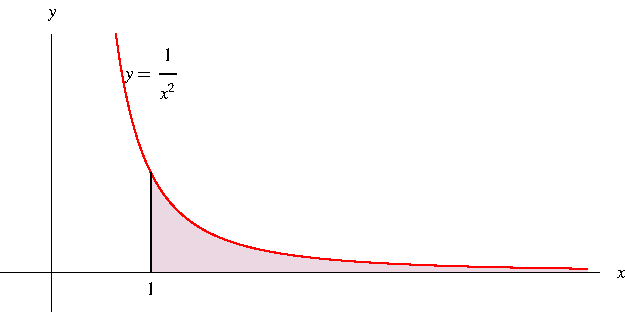
\includegraphics[height=3cm]{improper-integrals/pictures/08-08-xsquaredy.pdf}%
}%
\only<handout:0| 2-3>{%
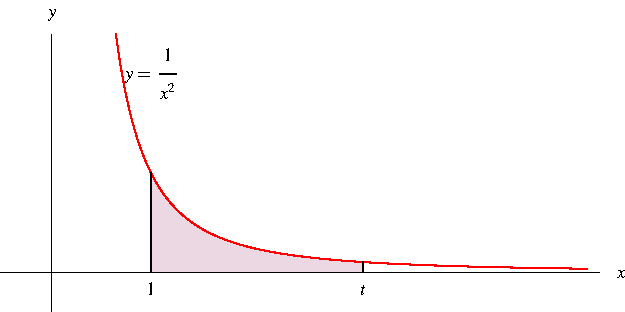
\includegraphics[height=3cm]{improper-integrals/pictures/08-08-xsquaredz.pdf}%
}%
\only<handout:0| 4-8>{%
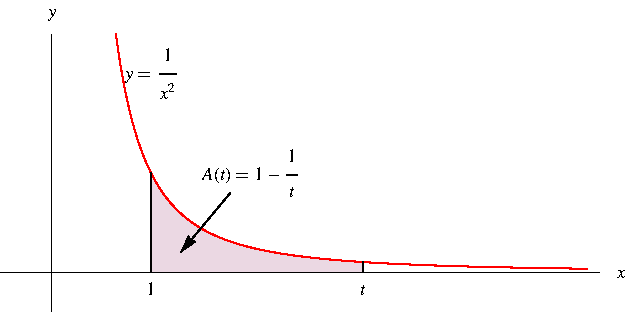
\includegraphics[height=3cm]{improper-integrals/pictures/08-08-xsquareda.pdf}%
}%
\only<handout:0| 9>{%
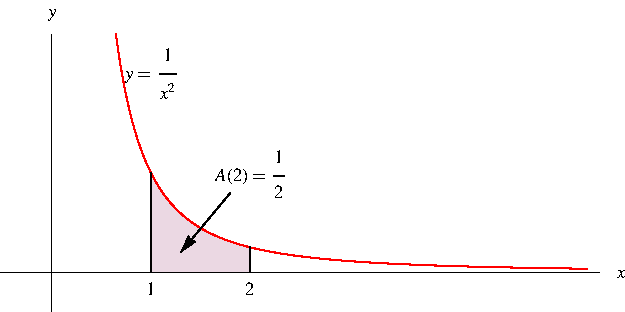
\includegraphics[height=3cm]{improper-integrals/pictures/08-08-xsquaredb.pdf}%
}%
\only<handout:0| 10>{%
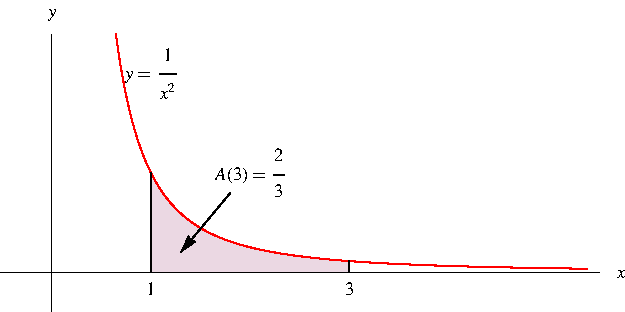
\includegraphics[height=3cm]{improper-integrals/pictures/08-08-xsquaredc.pdf}%
}%
\only<handout:0| 11>{%
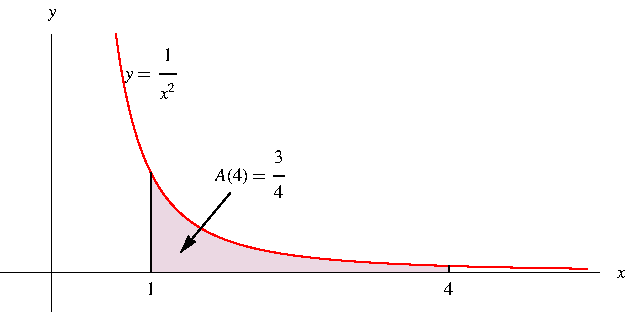
\includegraphics[height=3cm]{improper-integrals/pictures/08-08-xsquaredd.pdf}%
}%
\only<handout:0| 12>{%
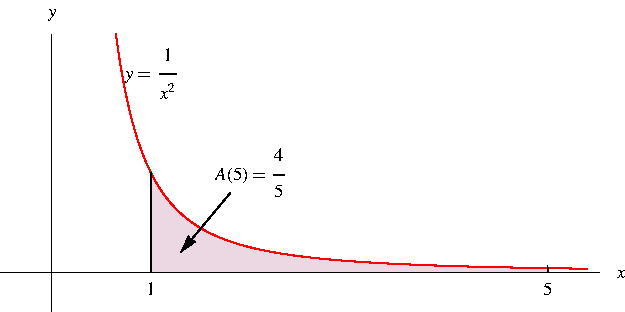
\includegraphics[height=3cm]{improper-integrals/pictures/08-08-xsquarede.pdf}%
}%
\only<handout:0| 13->{%
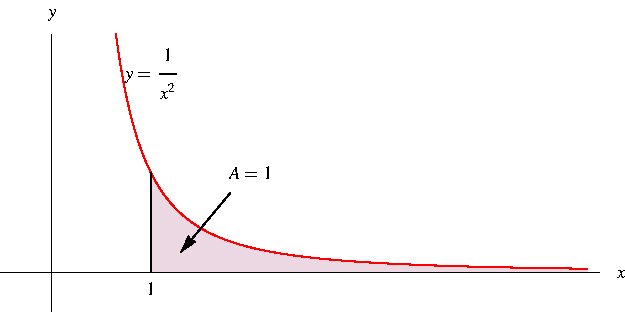
\includegraphics[height=3cm]{improper-integrals/pictures/08-08-xsquaredf.pdf}%
}%
\end{columns}
\begin{itemize}
\item<5->  Notice $A(t) < 1$ no matter how big $t$ is.
\item<6->  Also notice $\lim_{t\rightarrow \infty}A(t) = \alert<handout:0| 7-8>{\lim_{t\rightarrow \infty}\left( 1 - \frac{1}{t}\right) = \uncover<8->{1}}$\uncover<8->{.}
\item<14->  We say that the area $A$ is equal to $1$ and write $\int_1^\infty \frac{1}{x^2}\diff x = \lim_{t\rightarrow \infty}\int_1^t \frac{1}{x^2}\diff x = 1$.
\end{itemize}
\end{frame}
% end module improper-integral-geometry
